%% BioMed_Central_Tex_Template_v1.06
%%                                      %
%  bmc_article.tex            ver: 1.06 %
%                                       %

%%IMPORTANT: do not delete the first line of this template
%%It must be present to enable the BMC Submission system to
%%recognise this template!!

%%%%%%%%%%%%%%%%%%%%%%%%%%%%%%%%%%%%%%%%%
%%                                     %%
%%  LaTeX template for BioMed Central  %%
%%     journal article submissions     %%
%%                                     %%
%%          <8 June 2012>              %%
%%                                     %%
%%                                     %%
%%%%%%%%%%%%%%%%%%%%%%%%%%%%%%%%%%%%%%%%%


%%%%%%%%%%%%%%%%%%%%%%%%%%%%%%%%%%%%%%%%%%%%%%%%%%%%%%%%%%%%%%%%%%%%%
%%                                                                 %%
%% For instructions on how to fill out this Tex template           %%
%% document please refer to Readme.html and the instructions for   %%
%% authors page on the biomed central website                      %%
%% http://www.biomedcentral.com/info/authors/                      %%
%%                                                                 %%
%% Please do not use \input{...} to include other tex files.       %%
%% Submit your LaTeX manuscript as one .tex document.              %%
%%                                                                 %%
%% All additional figures and files should be attached             %%
%% separately and not embedded in the \TeX\ document itself.       %%
%%                                                                 %%
%% BioMed Central currently use the MikTex distribution of         %%
%% TeX for Windows) of TeX and LaTeX.  This is available from      %%
%% http://www.miktex.org                                           %%
%%                                                                 %%
%%%%%%%%%%%%%%%%%%%%%%%%%%%%%%%%%%%%%%%%%%%%%%%%%%%%%%%%%%%%%%%%%%%%%

%%% additional documentclass options:
%  [doublespacing]
%  [linenumbers]   - put the line numbers on margins

%%% loading packages, author definitions

%\documentclass[twocolumn]{bmcart}% uncomment this for twocolumn layout and comment line below
\documentclass{bmcart}

%%% Load packages
%\usepackage{amsthm,amsmath}
%\RequirePackage{natbib}
%\RequirePackage[authoryear]{natbib}% uncomment this for author-year bibliography
\RequirePackage{hyperref}
\usepackage[utf8]{inputenc} %unicode support
%\usepackage[applemac]{inputenc} %applemac support if unicode package fails
%\usepackage[latin1]{inputenc} %UNIX support if unicode package fails
\usepackage{footnote}
\usepackage{siunitx}
\sisetup{range-phrase = \text{--}}
\usepackage{float} % here for H placement parameter
\usepackage{tabularx}
\usepackage{colortbl}
\usepackage{xcolor}
\definecolor{evagrey}{RGB}{128,128,128}

% add path
\usepackage{placeins}
\usepackage{graphicx}
\graphicspath{{/Users/evayap/Documents/masters_thesis/bmc_template/figure_final/}}


%%%%%%%%%%%%%%%%%%%%%%%%%%%%%%%%%%%%%%%%%%%%%%%%%
%%                                             %%
%%  If you wish to display your graphics for   %%
%%  your own use using includegraphic or       %%
%%  includegraphics, then comment out the      %%
%%  following two lines of code.               %%
%%  NB: These line *must* be included when     %%
%%  submitting to BMC.                         %%
%%  All figure files must be submitted as      %%
%%  separate graphics through the BMC          %%
%%  submission process, not included in the    %%
%%  submitted article.                         %%
%%                                             %%
%%%%%%%%%%%%%%%%%%%%%%%%%%%%%%%%%%%%%%%%%%%%%%%%%


%% \def\includegraphic{}
%% \def\includegraphics{}



%%% Put your definitions there:
\startlocaldefs
\endlocaldefs


%%% Begin ...
\begin{document}

%%% Start of article front matter
\begin{frontmatter}

\begin{fmbox}
\dochead{Research}

%%%%%%%%%%%%%%%%%%%%%%%%%%%%%%%%%%%%%%%%%%%%%%
%%                                          %%
%% Enter the title of your article here     %%
%%                                          %%
%%%%%%%%%%%%%%%%%%%%%%%%%%%%%%%%%%%%%%%%%%%%%%

\title{True Positive Rate of Germline Variant Calling in Formalin-fixed Paraffin-embedded Tumours}

%%%%%%%%%%%%%%%%%%%%%%%%%%%%%%%%%%%%%%%%%%%%%%
%%                                          %%
%% Enter the authors here                   %%
%%                                          %%
%% Specify information, if available,       %%
%% in the form:                             %%
%%   <key>={<id1>,<id2>}                    %%
%%   <key>=                                 %%
%% Comment or delete the keys which are     %%
%% not used. Repeat \author command as much %%
%% as required.                             %%
%%                                          %%
%%%%%%%%%%%%%%%%%%%%%%%%%%%%%%%%%%%%%%%%%%%%%%

\author[
   addressref={aff1},                   % id's of addresses, e.g. {aff1,aff2}
   % noteref={n1},                        % id's of article notes, if any
   email={eyap@bcgsc.ca}   % email address
]{\inits{SQ}\fnm{Shyong Quin} \snm{Yap}}
\author[
   addressref={aff1,aff2},
	 corref={aff1},                       % id of corresponding address, if any
   email={akarsan@bcgsc.ca}
]{\inits{A}\fnm{Aly} \snm{Karsan}}

%%%%%%%%%%%%%%%%%%%%%%%%%%%%%%%%%%%%%%%%%%%%%%
%%                                          %%
%% Enter the authors' addresses here        %%
%%                                          %%
%% Repeat \address commands as much as      %%
%% required.                                %%
%%                                          %%
%%%%%%%%%%%%%%%%%%%%%%%%%%%%%%%%%%%%%%%%%%%%%%

\address[id=aff1]{%                           % unique id
  \orgname{British Columbia Cancer Research Centre}, % university, etc
  \street{675 West 10th Ave},                     %
  \postcode{V5Z 1L3}                              % post or zip code
  \city{Vancouver, BC},                           % city
  \cny{Canada}                                    % country
}
\address[id=aff2]{%
  \orgname{Department of Pathology and Laboratory Medicine, University of British Columbia},
  \street{Random Street},
  \postcode{Random Post Code}
  \city{Vancouver, BC},
  \cny{Canada}
}

%%%%%%%%%%%%%%%%%%%%%%%%%%%%%%%%%%%%%%%%%%%%%%
%%                                          %%
%% Enter short notes here                   %%
%%                                          %%
%% Short notes will be after addresses      %%
%% on first page.                           %%
%%                                          %%
%%%%%%%%%%%%%%%%%%%%%%%%%%%%%%%%%%%%%%%%%%%%%%

\begin{artnotes}
%\note{Sample of title note}     % note to the article
%\note[id=n1]{Equal contributor} % note, connected to author
\end{artnotes}

\end{fmbox}% comment this for two column layout

%%%%%%%%%%%%%%%%%%%%%%%%%%%%%%%%%%%%%%%%%%%%%%
%%                                          %%
%% The Abstract begins here                 %%
%%                                          %%
%% Please refer to the Instructions for     %%
%% authors on http://www.biomedcentral.com  %%
%% and include the section headings         %%
%% accordingly for your article type.       %%
%%                                          %%
%%%%%%%%%%%%%%%%%%%%%%%%%%%%%%%%%%%%%%%%%%%%%%

\begin{abstractbox}

\begin{abstract} % abstract
\parttitle{Background} %if any
The tumour genome contains germline information that may have clinical implications for patients and their families. Therefore, clinical laboratories must be equipped to confirm potential germline variants identified by routine tumour sequencing through downstream germline testing. The most common source of DNA in clinical laboratories is formalin-fixed paraffin-embedded (FFPE) tissues. However, fixation with formalin is known to cause DNA fragmentation and sequence artifacts that impose technical challenges in DNA sequencing.

Using amplicon sequencing data from FFPE tumours with matched blood specimens, we compared efficiency of amplicon generation and sequencing results between specimen types to characterize formalin-induced DNA damages. We determined the true positive rate of detecting germline variants in FFPE tumours by assessing the concordance of germline variants between blood and FFPE specimens. We also compared sensitivity of germline variant calling in FFPE tumours to blood at various variant allele frequency thresholds and established a cut-off to achieve high positive predictive value for referral of potential germline variants for confirmatory germline testing without compromising sensitivity of detection.

\parttitle{Results} %if any

\parttitle{Conclusions} %if any


\end{abstract}

%%%%%%%%%%%%%%%%%%%%%%%%%%%%%%%%%%%%%%%%%%%%%%
%%                                          %%
%% The keywords begin here                  %%
%%                                          %%
%% Put each keyword in separate \kwd{}.     %%
%%                                          %%
%%%%%%%%%%%%%%%%%%%%%%%%%%%%%%%%%%%%%%%%%%%%%%

\begin{keyword}
\kwd{Germline variants}
\kwd{Formalin-fixed paraffin-embedded tumours}
\kwd{Amplicon-based targeted next-generation sequencing}
\end{keyword}

% MSC classifications codes, if any
%\begin{keyword}[class=AMS]
%\kwd[Primary ]{}
%\kwd{}
%\kwd[; secondary ]{}
%\end{keyword}

\end{abstractbox}
%
%\end{fmbox}% uncomment this for twcolumn layout

\end{frontmatter}

%%%%%%%%%%%%%%%%%%%%%%%%%%%%%%%%%%%%%%%%%%%%%%
%%                                          %%
%% The Main Body begins here                %%
%%                                          %%
%% Please refer to the instructions for     %%
%% authors on:                              %%
%% http://www.biomedcentral.com/info/authors%%
%% and include the section headings         %%
%% accordingly for your article type.       %%
%%                                          %%
%% See the Results and Discussion section   %%
%% for details on how to create sub-sections%%
%%                                          %%
%% use \cite{...} to cite references        %%
%%  \cite{koon} and                         %%
%%  \cite{oreg,khar,zvai,xjon,schn,pond}    %%
%%  \nocite{smith,marg,hunn,advi,koha,mouse}%%
%%                                          %%
%%%%%%%%%%%%%%%%%%%%%%%%%%%%%%%%%%%%%%%%%%%%%%

%%%%%%%%%%%%%%%%%%%%%%%%% start of article main body
% <put your article body there>

%%%%%%%%%%%%%%%%
%% Background %%
%%
\section*{Background}

The application of next-generation sequencing (NGS) technologies for tumour profiling has been increasingly integrated into oncologic care to detect targetable somatic mutations and personalize treatments for cancer patients. Although analysis of tumour-normal paired samples is required to accurately discriminate between somatic and germline variants, most clinical laboratories only sequence tumour samples to minimize cost and turnaround time \cite{Raymond2016}. However, genomic analyses of tumours can also reveal secondary genomic findings, which are germline information that may have clinical implications for patients and their family members \cite{Raymond2016}. In fact, several studies demonstrated that a germline cancer-predisposing variant is present in 3-10\% of patients undergoing tumour-normal sequencing \cite{Raymond2016,Meric-Bernstam2016,Schrader2015,Jones2015}. Therefore, clinical laboratories providing tumour genomic testing must be equipped to perform germline confirmatory testing on potential germline variants or be prepared to refer such cases to external services.

Because the tumour genome contains germline information, clinical laboratories can leverage tumour genomic testing to perform initial screening for clinically relevant germline variants such as variants in pharmacogenomic (PGx) genes. Subsequently, a similar framework for validating secondary germline findings can be applied, in which only patients with potential germline PGx variants are subjected to downstream germline testing. This procedure for germline PGx testing is more cost-effective because it does not require processing, sequencing, and analysis of normal DNA for every patient. The ability to implement germline PGx testing at a reduced cost can significantly benefit patient care because these variants cause functional changes in drug targets and drug disposition proteins (proteins involved in drug metabolism and transport), thereby contributing to inter-patient differences in chemotherapeutic response \cite{McLeod2013}. Hence, such genomic information can be used to guide the selection of chemotherapeutic drugs and optimization of drug dosage for cancer patients, leading to improved safety and efficacy of treatment and reduced risk of toxicity \cite{McLeod2013}.

Detection of genomic alterations in tumour DNA is also faced with technical challenges conferred by formalin-fixed paraffin-embedded (FFPE) tumour specimens \cite{Do2015,Wong2014}. Tumour biopsies are often formalin-fixed to preserve tissue morphology for histological examination and to enable storage at room temperature; however, formalin fixation causes DNA fragmentation and base modifications, which pose difficulties in using DNA extracted from FFPE tumours for clinical genomic testing \cite{Do2015,Wong2014}. Fragmentation damage caused by formalin fixation leads to reduced template DNA for PCR amplification, thereby affecting the efficiency of amplicon-based NGS testing \cite{Do2015,Wong2014}. Furthermore, the degree of DNA fragmentation was shown to be higher in tissues from older FFPE blocks and tissues fixed with formalin of lower pH \cite{Do2015}. Formalin fixation is also problematic because it gives rise to depurination, which generates abasic sites, and cytosine deamination resulting in C$>$T/G$>$A transitions \cite{Do2015}. These forms of formalin-induced DNA damage contribute to the presence of sequence artifacts in FFPE specimens, which can be inaccurately identified as real genomic alterations.

In this study, we assessed the concordance of germline PGx variants between tumour and matched normal DNA by analyzing amplicon-based targeted NGS data from 213 patients with tumour-normal paired samples. While matched normal DNA was derived from peripheral blood, tumour DNA was extracted from FFPE tumour blocks; thus, we compared the quality metrics of sequencing data between tumour and blood specimens and evaluated the prevalence of formalin-induced DNA damages to address the impact of formalin fixation on amplicon-based NGS testing. We demonstrated that germline PGx variants can be identified with high sensitivity and precision in FFPE tumour DNA using a clinical targeted sequencing panel.

%\cite{koon,oreg,khar,zvai,xjon,schn,pond,smith,marg,hunn,advi,koha,mouse}

\section*{Methods}

\subsection*{Patient Samples}
Blood and FFPE tumour specimens were acquired from 213 patients who provided informed consent for The OncoPanel Pilot (TOP) study, a pilot study to optimize the OncoPanel, which is an amplicon-based targeted NGS panel for solid tumours, and assess its application for guiding disease management and therapeutic intervention. Patients in the TOP study are those with advanced cancers including colorectal cancer, lung cancer, melanoma, gastrointestinal stromal tumour (GIST), and other cancers (\autoref{cancertypes}). The age of paraffin block for tumour specimens ranges from 18 to 5356 days with a median of 274 days.

\begin{table}[H]
\caption{Distribution of cancer types in the TOP cohort.}\label{cancertypes}
      \begin{tabular}{lccc}
        \hline
        Cancer Type & Number of Cases & Percentage (\%) \\ \hline
        Colorectal & 97 & 46 \\
        Lung & 59 & 28 \\
        Melanoma & 18 & 8 \\
				Other* & 17 & 8 \\
				GIST & 7 & 3 \\
				Sarcoma & 4 & 2 \\
				Neuroendocrine & 4 & 2 \\
				Cervical & 2 & 0.9 \\
				Ovarian & 2 & 0.9 \\
				Breast & 2 & 0.9 \\
				Unknown & 1 & 0.5 \\ \hline
      \end{tabular} \\
\raggedright
{\small *This category includes thyroid, peritoneum, lung sarcomatoid carcinoma, Fallopian tube, gastric, endometrial, squamous cell carcinoma, anal, salivary gland, peritoneal epithelial mesothelioma, adenoid cystic carcinoma, pancreas, breast, gall bladder, parotid epithelial myoepithelial carcinoma, and small bowel cancers.}
\end{table}

\subsection*{OncoPanel (Solid Tumour NGS Panel)}
The OncoPanel is offered by the British Columbia Cancer Agency (BCCA) for clinical genomic testing of coding exons and clinically relevant hotpots of 20 cancer-related genes and six PGx genes: \textit{DPYD}, \textit{GSTP1}, \textit{MTHFR}, \textit{TYMP}, \textit{TYMS}, and \textit{UGT1A1}. Full list of genes and gene reference models for the OncoPanel is presented in \autoref{genemodel}. Primers were designed by RainDance Technologies (Lexington, MA) using the GRCh37/hg19 reference sequence to generate 416 amplicons between 100 bp and 250 bp in size, which interrogate $\sim$ 20 kb of target bases. Target regions of the six PGx genes in the OncoPanel were assayed by 49 out of 416 amplicons. Complete lists of primers and amplicons are provided in the Supplemental Materials.

\subsection*{Sample Preparation, Library Construction, and Illumina Sequencing}
Genomic DNA was extracted from blood and FFPE tumour specimens using the Gentra Autopure LS DNA preparation platform and QIAamp DNA FFPE tissue kit (Qiagen, Hilden, Germany) respectively. The extracted DNA was sheared according to a previously described protocol \cite{Bosdet2013} to attain approximate sizes of 3 kb followed by PCR primer merging, amplification of target regions, and adapter ligation using the Thunderstorm NGS Targeted Enrichment System (RainDance Technologies, Lexington, MA) as per manufacturer's protocol. Barcoded amplicons were sequenced with the Illumina MiSeq system for paired end sequencing with a v2 250-bp kit (Illumina, San Diego, CA).

\subsection*{Variant Calling Pipeline}
Reads that passed the Illumina Chastity filter were aligned to the GRCh37/hg19 human reference genome using the BWA mem algorithm (version 0.5.9) with default parameters, and the alignments were processed and converted to the BAM format using SAMtools (version 0.1.18). Variant calling was performed with the SAMtools \texttt{mpileup} function \texttt{(samtools mpileup -BA -d 500000 -L 500000 -q 1)} to generate pileup files for all target bases followed by the VarScan2 \texttt{mpileup2cns} (version 2.3.6) function with parameter thresholds of variant allele frequency $\geq$ 10\% and Phred-scaled base quality score $\geq$20 \texttt{(--min-var-freq 0.1 --p-value 0.01 --strand-filter 0 --output-vcf --variants --min-avg-qual 20)}. Variant calls were filtered using the VarScan2 \texttt{fpfilter} function with fraction of variant reads from each strand $\geq$ 0.1 and default thresholds for other parameters. SnpEff (version 4.2) was used for variant annotation and effect prediction whereas the SnpSift package in SnpEff was used to annotate variants with databases such as dbSNP (b138), COSMIC (version 70), 1000 Genomes Project, ClinVar, and ExAC (release 0.3) for interpretation.

\subsection*{Data Analysis}
More details \ldots

\newpage
%%%%%%%%%%%%%%%%%%%%%%%%%%%%%%%%%%%%%%%%%%%%%%%%%%%%%%%%%%%%%%%%%%%%%
\section*{Results}
%%%%%%%%%%%%%%%%%%%%%%%%%%%%%%%%%%%%%%%%%%%%%%%%%%%%%%%%%%%%%%%%%%%%%
\subsection*{Comparison of amplicon generation and sequencing metrics between blood and FFPE specimens}

\begin{figure}[!htb]
	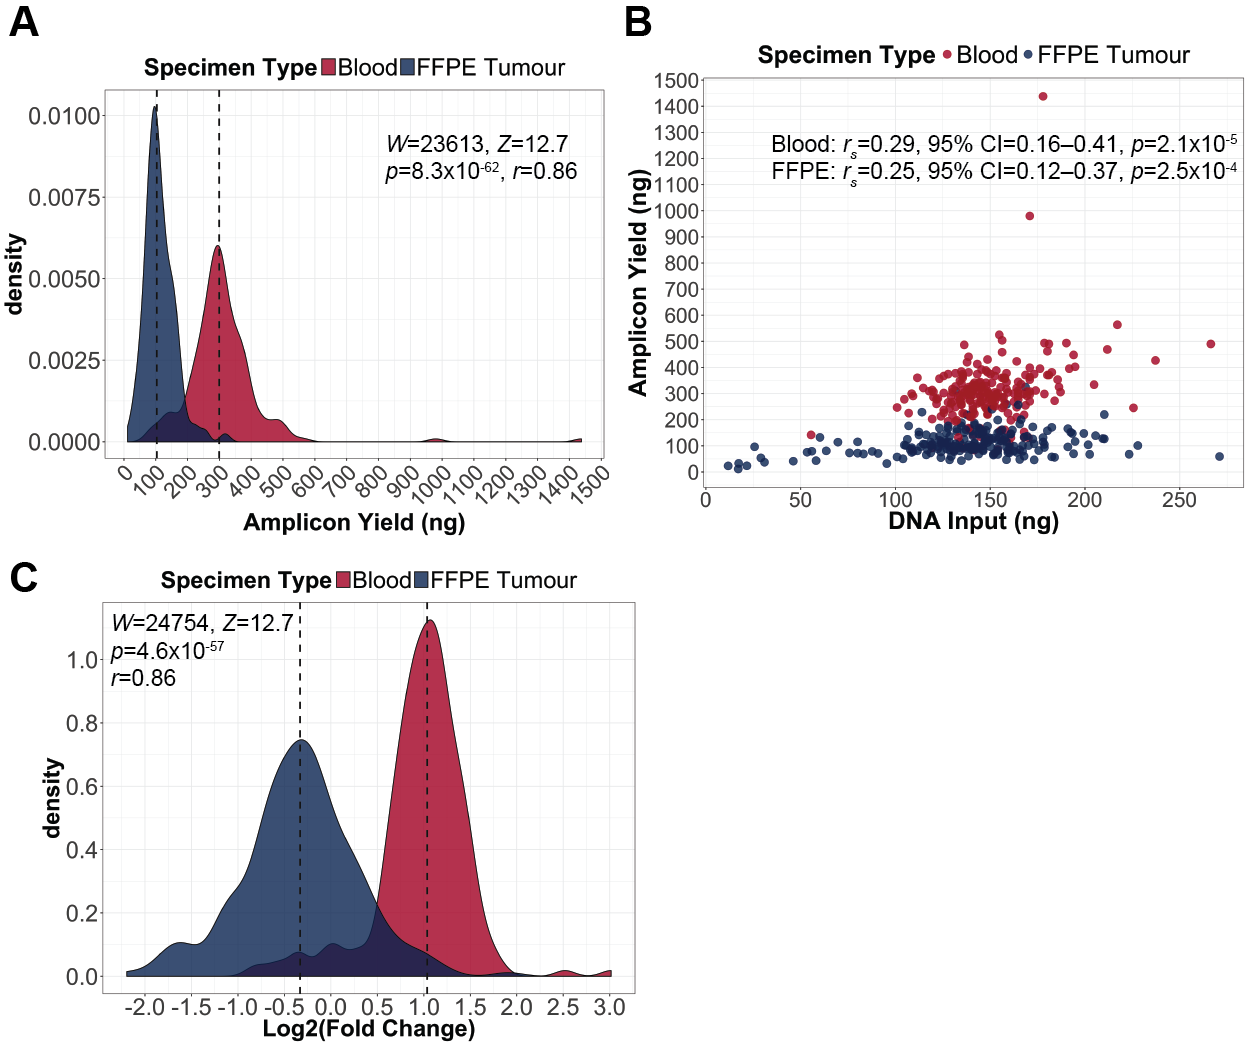
\includegraphics[scale=0.6]{dna_input_amp_yield.png}
	\caption{Assessment of amplicon generation and sequencing results in blood and FFPE specimens. (A) Amplicon yield and DNA input for amplicon generation are weakly correlated in blood and FFPE specimens as demonstrated by Spearman's rank correlation (\textit{p} $<$ 0.05). (B) Amplicon yield is significantly lower in FFPE specimens than blood based on the Wilcoxon signed-rank test (\textit{p} $<$ 0.05). (C) Percentage of target bases is significantly different between blood and FFPE specimens at all coverage thresholds as demonstrated by the Wilcoxon signed-rank test (****\textit{p} $<$ 0.0001; **\textit{p} $<$ 0.01; na = not available). Box plots show the median (horizontal bar within) and interquartile range (IQR) of percentage of target bases that meet the respective coverage thresholds, with whiskers representing the range of data not exceeding 1.5x the IQR and circles indicating outliers. (D) Percentages of on-target and off-target aligned reads are not significantly different between specimen types as shown by the Wilcoxon signed-rank test, whereas percentages of unaligned and contaminant reads are significantly different (\textit{p} $<$ 0.05). Box plots show the median (horizontal bar within) and IQR of percentage of reads, with whiskers representing the range of data not exceeding 1.5x the IQR and circles indicating outliers.}
	\label{fig:dna_input_amp_yield}
\end{figure}
\FloatBarrier

\newpage
\begin{table}[H]
\caption{Comparison of amplicon generation and sequencing results between blood and FFPE specimens using the Wilcoxon signed-rank test.}\label{metrics}
\begin{tabular}{lllllll}
  \hline
  \multicolumn{1}{l}{ }
  &
  \multicolumn{2}{l}{Blood}
  &&
  \multicolumn{2}{l}{FFPE Tumour}
  &
  \multicolumn{1}{l}{ } \\
  \cline{2-3}\cline{5-6}
  Parameter & Median & Range && Median & Range & \textit{p} value ($<$ 0.05\textsuperscript{*})\\
  \hline
  DNA Input (ng) & 147.8 & 55.5--266.4 && 140.9 & 11.8--271.0 & \num{3.5e-4}\textsuperscript{*} \\
  Amplicon Yield (ng) & 299.2 & 84.0--1438.0 && 103.6 & 11.6--325.5 & \num{4.1e-37}\textsuperscript{*} \\
  Average Per Base & 1270 & 950--1519 && 1194 & 283--1405 & \num{1.7e-22}\textsuperscript{*} \\
  Normalized Coverage & & && & & \\
  $\geq$ 0x Target Bases (\%) & 100.0 & 100.0-100.0 && 100.0 & 97.0-100.0 &
  -- \\
  $\geq$ 100x Target Bases (\%) & 100.0 & 100.0-100.0 && 100.0 & 37.0--100.0 &
  \num{1.5e-3}\textsuperscript{*} \\
  $\geq$ 200x Target Bases (\%) & 100.0 & 100.0-100.0 && 100.0 & 29.0--100.0 &
  \num{1.4e-7}\textsuperscript{*} \\
  $\geq$ 300x Target Bases (\%) & 100.0 & 98.0-100.0 && 99.0 & 24.0--100.0 &
  \num{2.3e-16}\textsuperscript{*} \\
  $\geq$ 400x Target Bases (\%) & 99.0 & 94.0-100.0 && 97.0 & 17.0--100.0 &
  \num{2.0e-23}\textsuperscript{*} \\
  $\geq$ 500x Target Bases (\%) & 97.0 & 84.0-99.0 && 89.5 & 13.0--99.0 &
  \num{5.1e-29}\textsuperscript{*} \\
  $\geq$ 600x Target Bases (\%) & 92.0 & 77.0-97.0 && 87.0 & 9.0--96.0 &
  \num{3.0e-26}\textsuperscript{*} \\
  $\geq$ 700x Target Bases (\%) & 84.0 & 70.0-91.0 && 80.0 & 6.0--91.0 &
  \num{2.3e-21}\textsuperscript{*} \\
  $\geq$ 800x Target Bases (\%) & 77.0 & 63.0-84.0 && 73.0 & 5.0--83.0 &
  \num{6.0e-23}\textsuperscript{*} \\
  $\geq$ 900x Target Bases (\%) & 73.0 & 54.0-78.0 && 66.0 & 4.0--77.0 &
  \num{9.8e-30}\textsuperscript{*} \\
  $\geq$ 1000x Target Bases (\%) & 68.5 & 41.0-73.0 && 59.0 & 3.0-74.0 & \num{1.0e-30}\textsuperscript{*} \\
  On-target Aligned Reads (\%) & 86.8 & 74.0--95.9 && 88.4 & 32.5--97.4 & \num{0.094} \\
  Off-target Aligned Reads (\%) & 7.3 & 0.8-24.0 && 8.4 & 0.4--60.4 & \num{0.72} \\
  Unaligned Reads (\%) & 1.3 & 0.4--7.2 && 0.8 & 0.3--12.1 & \num{5.2e-15}\textsuperscript{*} \\
  Contaminant (\%) & 3.9 & 0.1--8.1 && 1.4 & 0.03--63.6 &
  \num{9.9e-4}\textsuperscript{*} \\
  \hline
\end{tabular} \\
\end{table}} \\
\end{table}

%%%%%%%%%%%%%%%%%%%%%%%%%%%%%%%%%%%%%%%%%%%%%%%%%%%%%%%%%%%%%%%%%%%%%
\subsection*{Reduced amplicon coverage in FFPE specimens is more profound for increased amplicon length}

\begin{figure}[!htb]
	\centering
	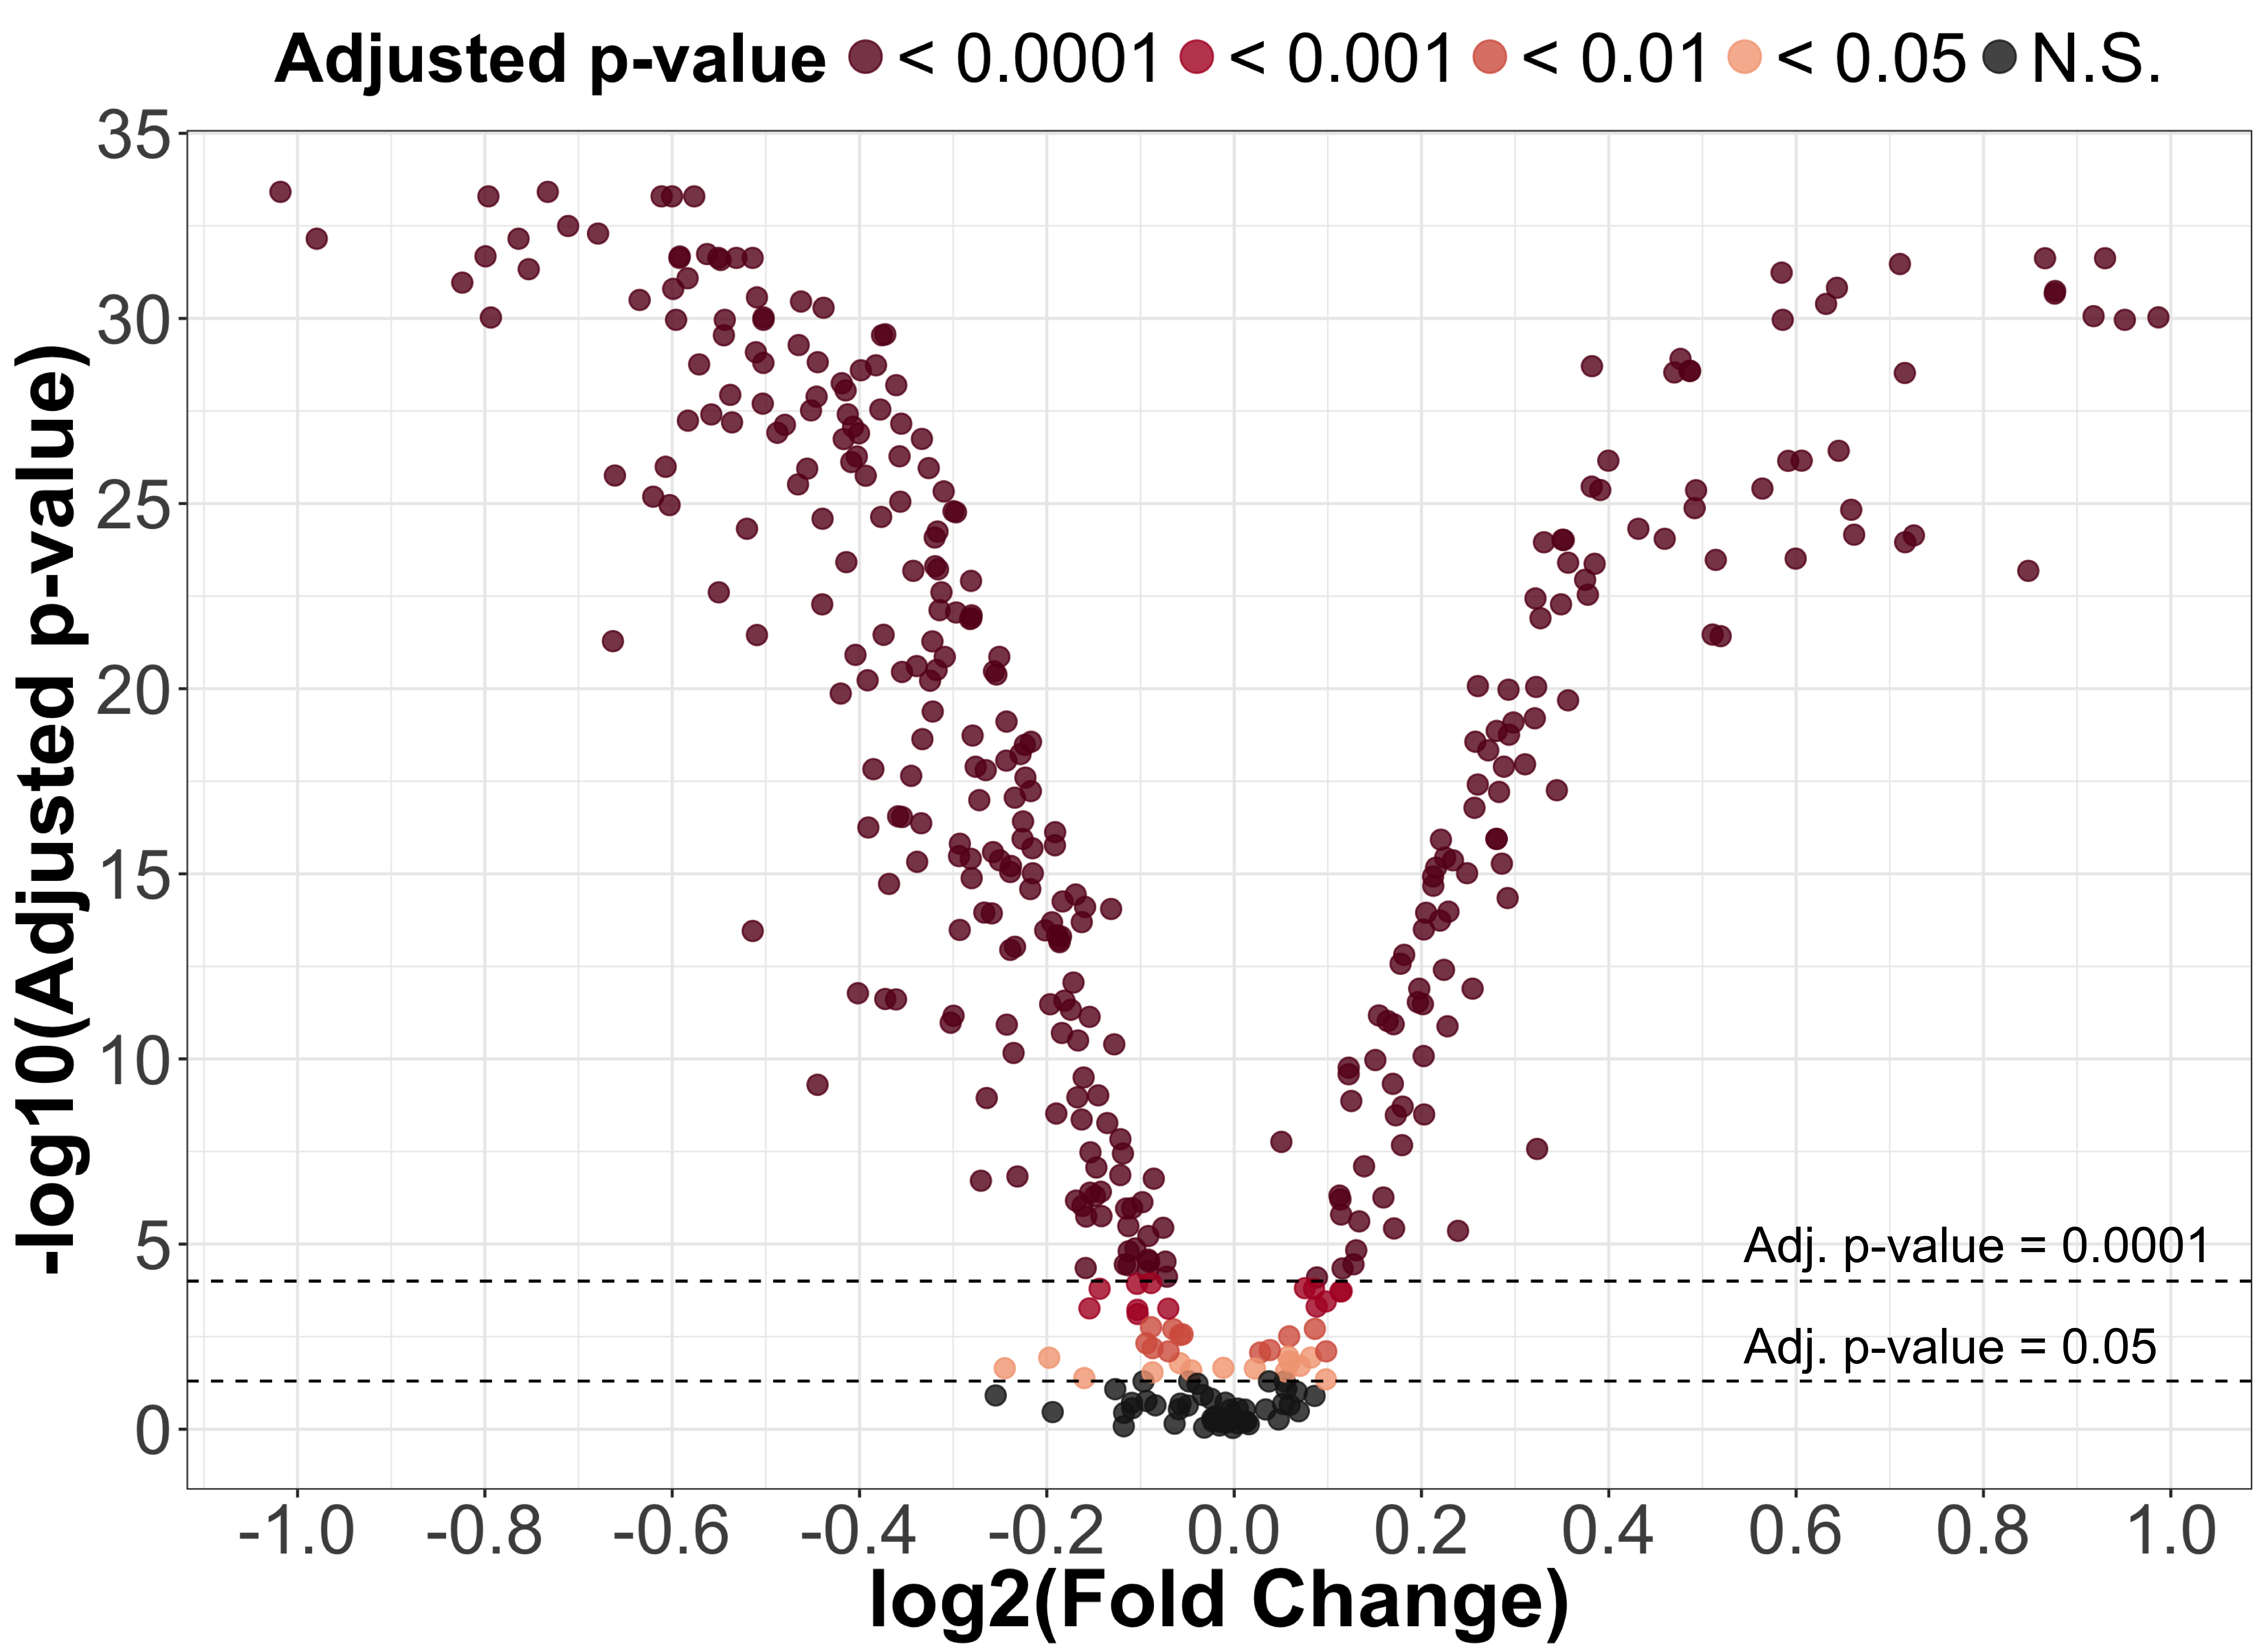
\includegraphics[scale=0.1]{amp_norm_depth_med_wilcoxon_volcano.png}
	\caption{Normalized coverage of amplicons is highly variable between blood and FFPE specimens. Wilcoxon signed-rank test with Benjamini-Hochberg multiple hypothesis testing correction showed significant differences in normalized coverage for the majority of amplicons (adjusted \textit{p}-value $<$ 0.05). Volcano plot illustrates the -log10 adjusted \textit{p}-values in relation to the log2 fold change between median normalized amplicon coverage in FFPE specimens and blood specimens.}
	\label{fig:amp_norm_depth_med_wilcoxon_volcano}
\end{figure}

\newpage
\begin{figure}[!htb]
	\centering
	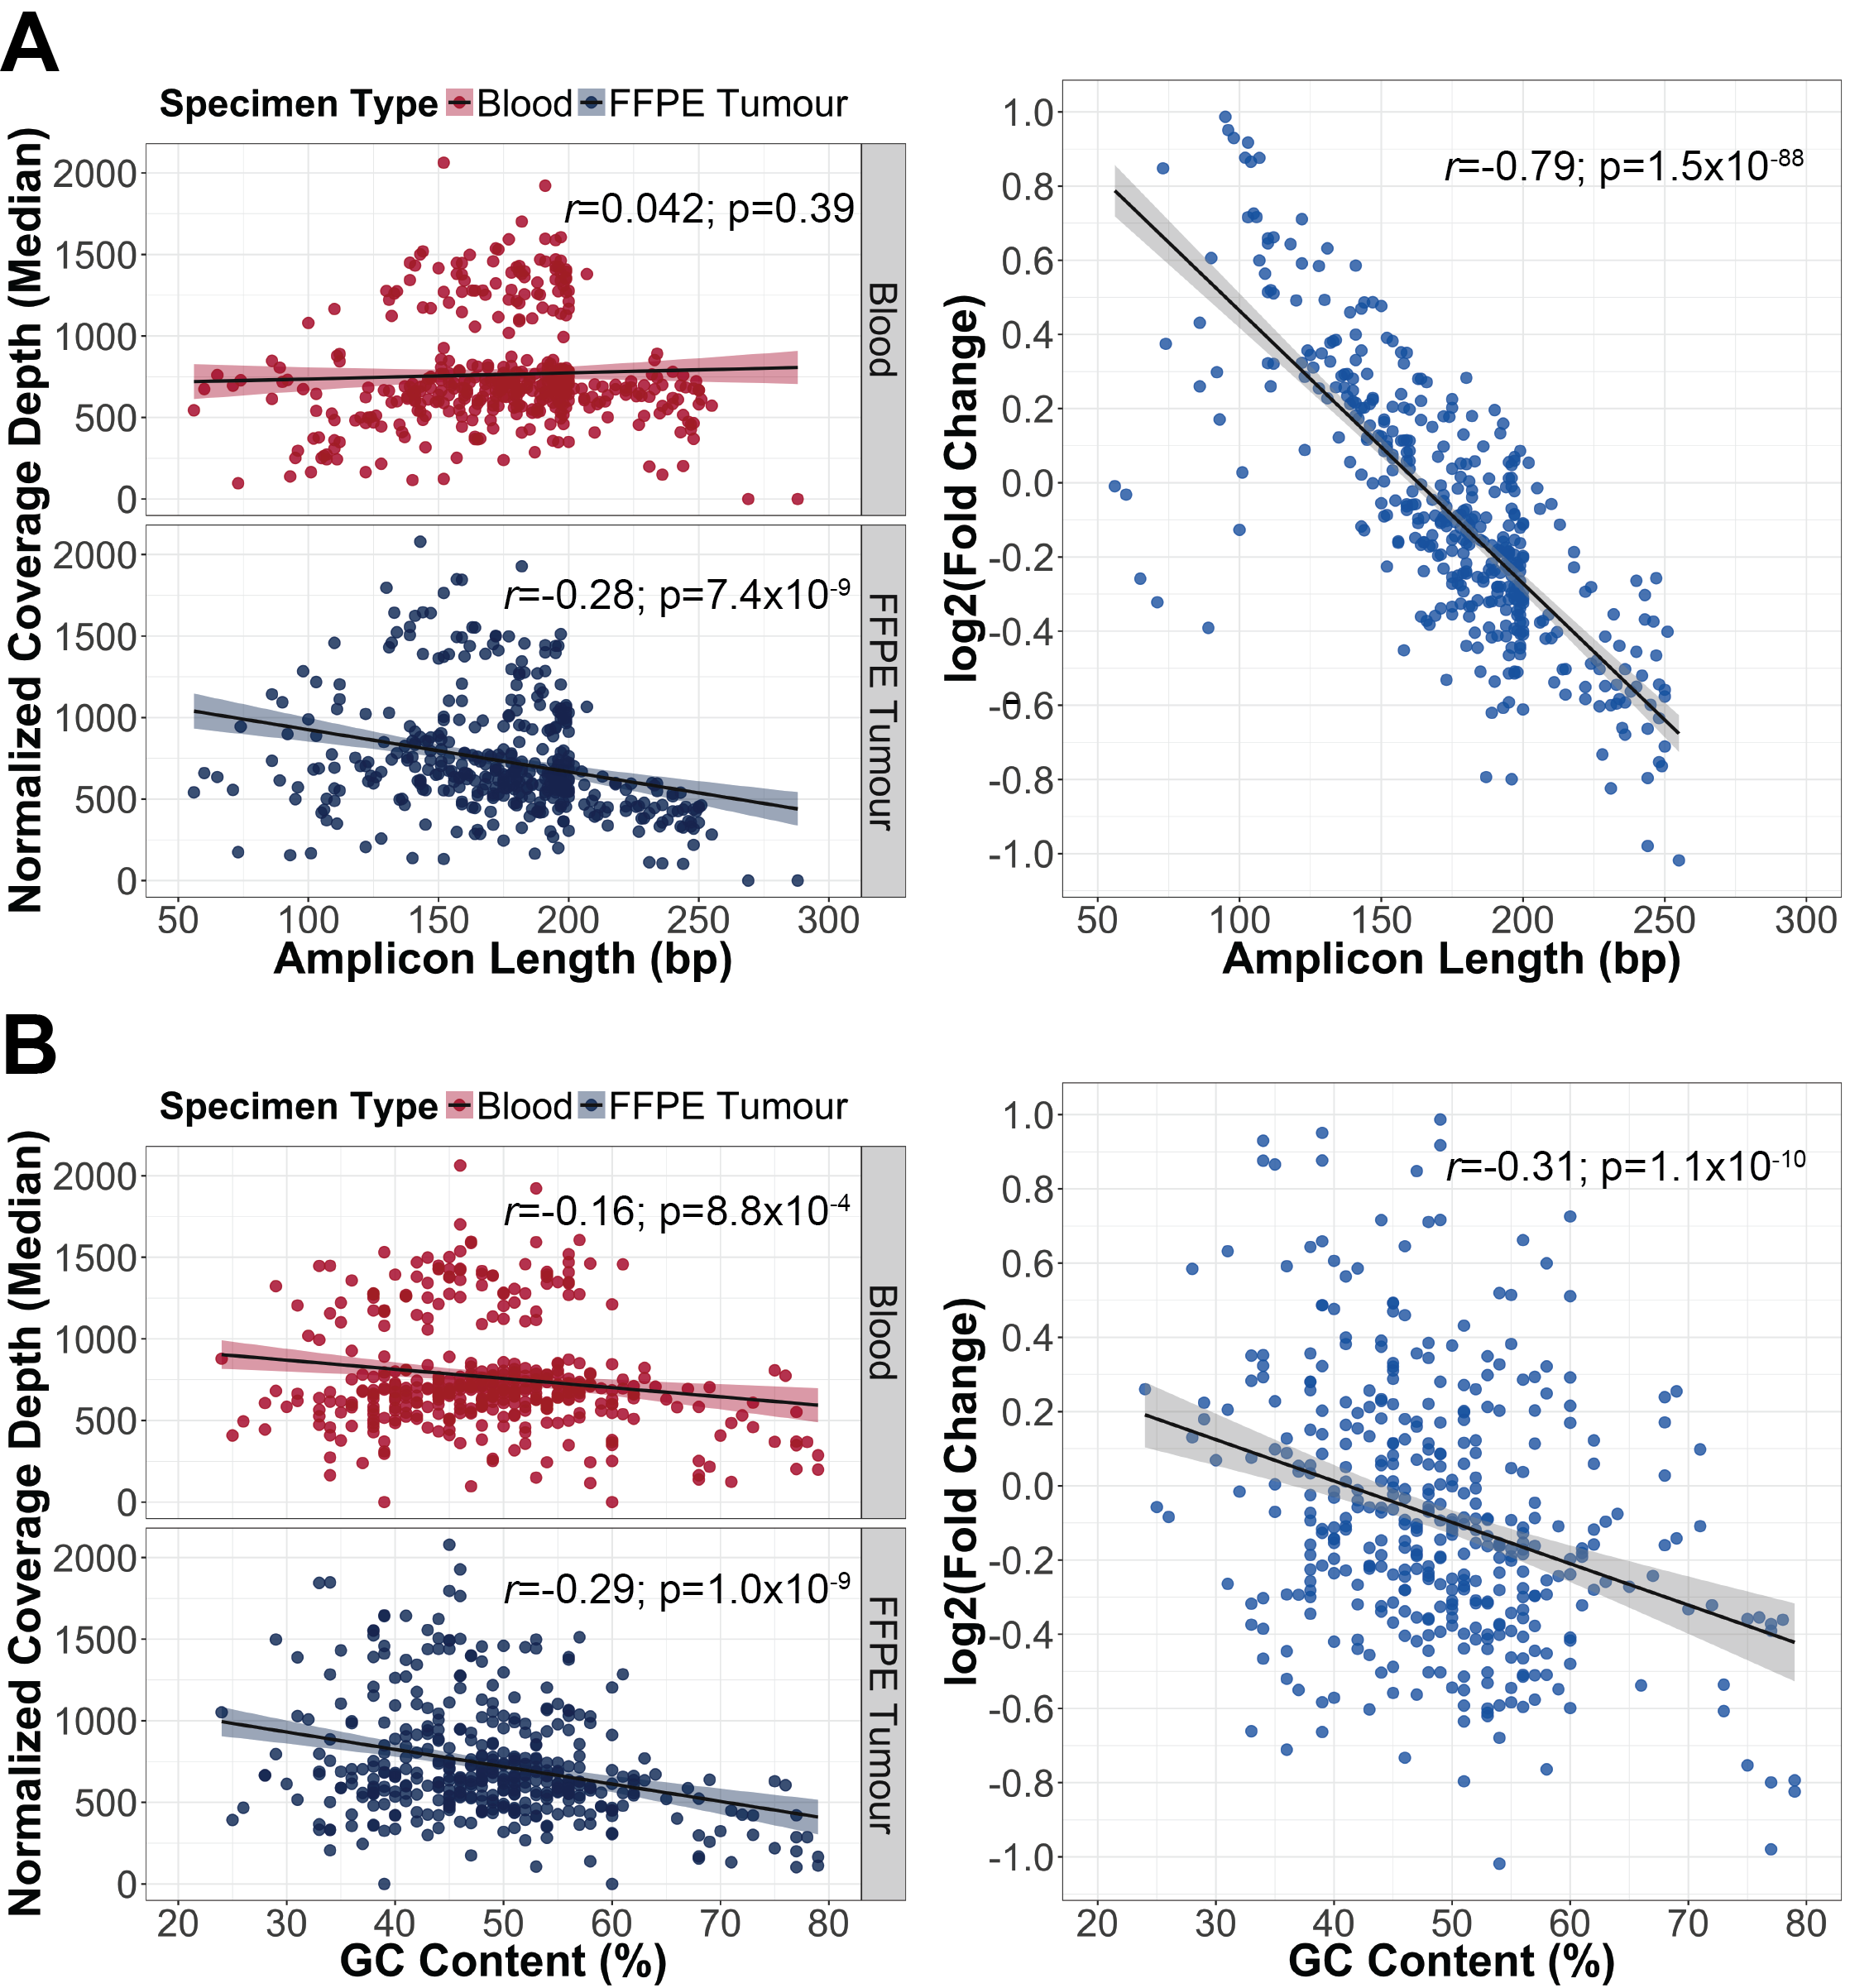
\includegraphics[scale=0.6]{amp_cov_lm.png}
	\caption{Amplicon length and GC content have significant effects on amplicon coverage depth. (A) Pearson's correlation demonstrated a significant negative correlation between normalized amplicon coverage depth and amplicon length in FFPE tumours, but not in blood (\textit{p}-value $<$ 0.05). Log2 fold change between the median amplicon coverage depth in FFPE specimens and blood was also negatively correlated with amplicon length as demonstrated by Pearson's correlation also showed a strong negative correlation between the change in amplicon coverage depth in FFPE specimens from that log2 fold change between median normalized amplicon coverage in FFPE specimens and blood specimens }
	\label{fig:amp_cov_lm}
\end{figure}

\begin{table}[H]
\caption{Multiple regression using amplicon length and GC content as predictors for log2 fold change between median normalized amplicon coverage in FFPE specimens and blood specimens.}
\label{multiple_regression}
\centering
      \begin{tabular}{l|ccccl}
        Variable & Unstandardized Coefficient & Standard Error & Standardized Coefficient & \textit{p}-value
        \\
        \hline
        Length (bp) & \num{-7.24e-3} & \num{2.54e-4} & \num{-7.75e-1} & \num{2.47e-99}
				\\
				GC Content (\%) & \num{-9.92e-3} & \num{9.77e-4} & \num{-2.77e-1} & \num{8.70e-22}
				\\
				\hline
				\\
				 & \multicolumn{4}{r}{Intercept = 1.66, Adjusted R\textsuperscript{2} = 0.695}
				\\
				 & \multicolumn{4}{r}{\textit{F}(2, 411) = 471, \textit{p}-value = \num{4.65e-107}}
				\\
				\hline
      \end{tabular} \\
\end{table}

\newpage
%%%%%%%%%%%%%%%%%%%%%%%%%%%%%%%%%%%%%%%%%%%%%%%%%%%%%%%%%%%%%%%%%%%%%
\subsection*{Deamination effects lead to increased C$>$T/G$>$A transitions at low allele frequency in FFPE specimens}

\begin{figure}[!htb]
	\centering
	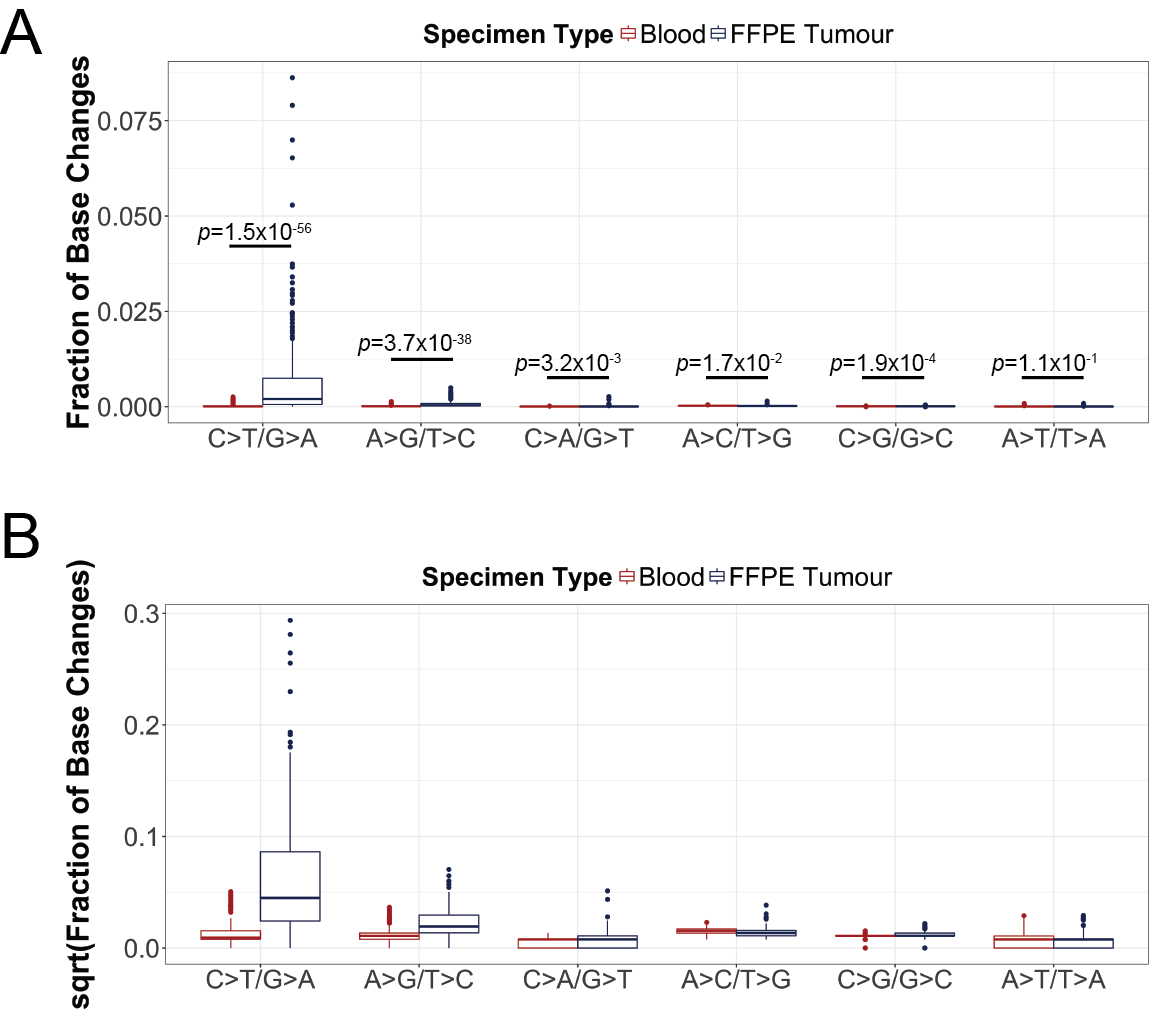
\includegraphics[scale=0.6]{deamination_effect_blood_ffpe.png}
	\caption{Add caption.}
	\label{fig:deamination_effect_blood_ffpe}
\end{figure}

\begin{table}[H]
\caption{Multiple pairwise comparison of log2 fold change of fraction of base changes in FFPE specimen over blood using Dunn's test with Benjamini-Hochberg multiple hypothesis testing correction. Top values represent Dunn's pairwise \textit{z} statistics, whereas bottom values represent adjusted \textit{p}-value. Asterisk(*) indicates significance level of adjusted \textit{p}-value $<$ 0.05.}
\label{dunntest}
\centering
      \begin{tabular}{r|l|l|l|l|ll}
        Type of Base Changes & A$>$C/T$>$G & A$>$G/T$>$C & A$>$T/T$>$A & C$>$A/G$>$T & C$>$G/G$>$C
        \\
        \hline
        A$>$G/T$>$C & -11.7 &  &  &  &
        \\
				 & \num{4.15e-31}\mbox{*} &  &  &  &
				\\
				\hline
        A$>$T/T$>$A & -0.399 & 9.57 &  &  &
        \\
				 & \num{3.45e-1} & \num{1.31e-21}\mbox{*} & & &
				\\
				\hline
        C$>$A/G$>$T & -3.46 & 6.39 & -2.73 &  &
        \\
				 & \num{4.00e-4}\mbox{*} & \num{1.52e-10}\mbox{*} & \num{3.99e-3}\mbox{*} & &
				\\
				\hline
        C$>$G/G$>$C & -3.02 & 8.63 & -2.17 & 0.918 &
				\\
				 & \num{1.73e-3}\mbox{*} & \num{6.76e-18}\mbox{*} & \num{1.71e-2}\mbox{*} & \num{1.92e-1} &
        \\
				\hline
        C$>$T/G$>$A & -17.1 & -5.60 & -14.3 & -11.1 & -14.1
        \\
				 & \num{7.78e-65}\mbox{*} & \num{1.76e-8}\mbox{*} & \num{5.10e-46}\mbox{*} & \num{1.32e-28}\mbox{*} & \num{6.46e-45}\mbox{*}
				 \\
				\hline
      \end{tabular} \\
\end{table}


\begin{figure}[!htb]
	\centering
	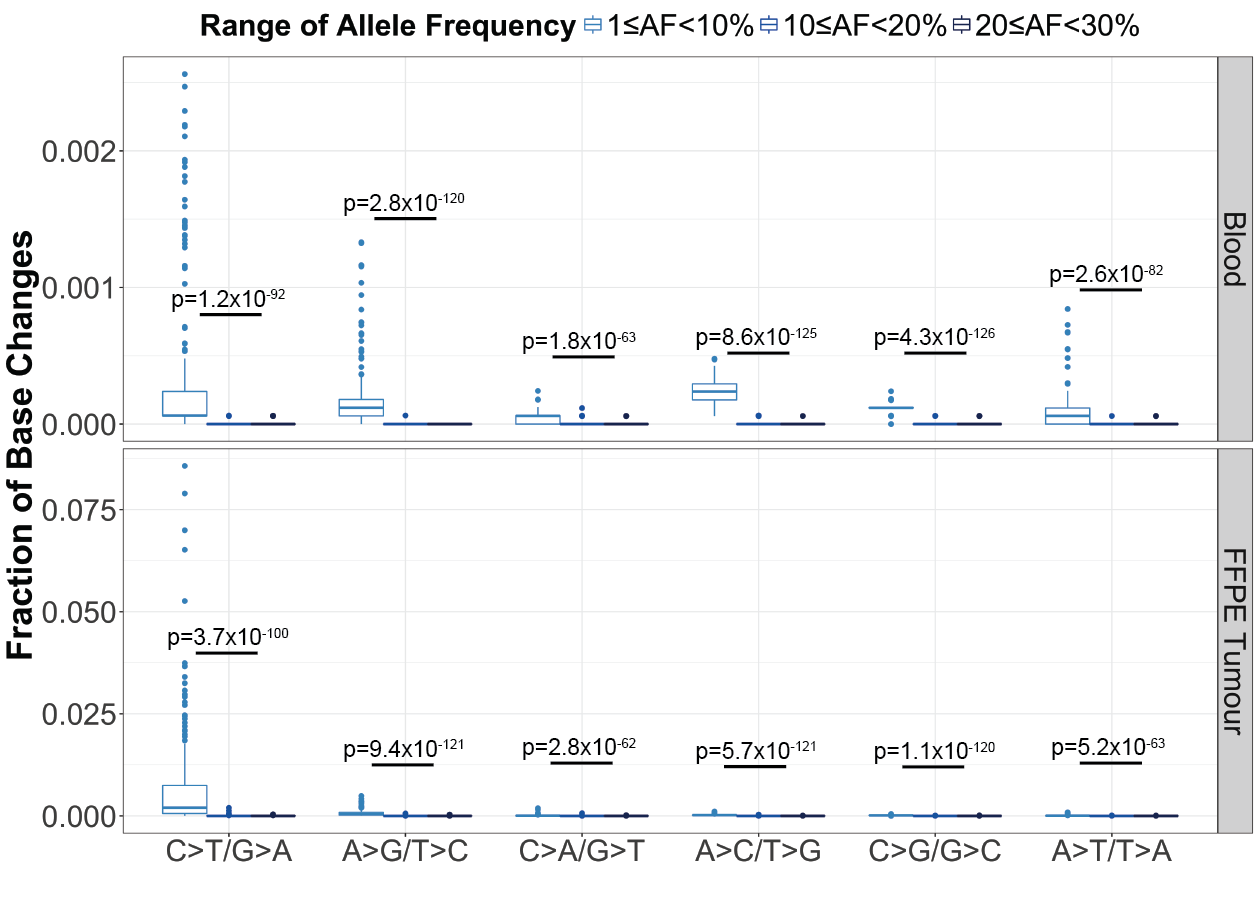
\includegraphics[scale=0.58]{deamination_effect_af_range.png}
	\caption{Add caption.}
	\label{fig:deamination_effect_af_range}
\end{figure}


%%%%%%%%%%%%%%%%%%%%%%%%%%%%%%%%%%%%%%%%%%%%%%%%%%%%%%%%%%%%%%%%%%%%%
\subsection*{Increased age of paraffin block results in reduced amplicon yield and elevated events of C$>$T/G$>$A sequence artifacts}

\begin{figure}[!h]
	\centering
	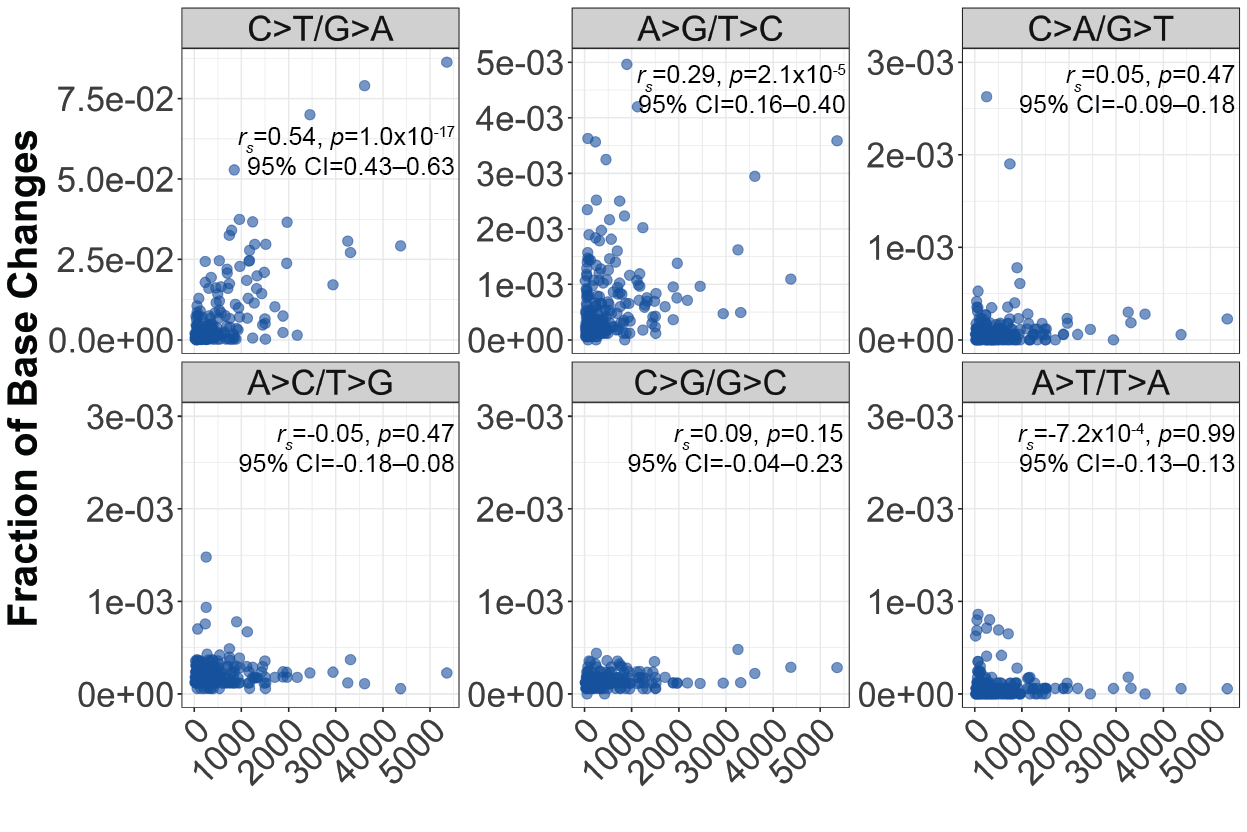
\includegraphics[scale=0.5]{deamination_effect_age.png}
	\caption{Add caption.}
	\label{fig:deamination_effect_age}
\end{figure}

\begin{table}[!h]
\caption{Determination of correlation between pre-sequencing variables and sequencing results using Spearman's correlation. Top values represent Spearman's \textit{rho} and 95\% confidence interval in brackets, whereas bottom values represent \textit{p}-value. Asterisk(*) indicates significance level of \textit{p}-value $<$ 0.05.}
\label{spearman_corr}
\centering
      \begin{tabular}{l|l|l|l|ll}
        Variable & Amplicon & Age of Paraffin & Fraction of & Average Per Base
        \\
				 & Yield (ng) & Block (Day) & C$>$T/G$>$A & Normalized Coverage
				\\
        \hline
        Age of Paraffin & -0.42 (-0.52-- -0.30) & & &
				\\
				Block (Day) & \num{5.2e-7}\mbox{*} & & &
        \\
				\hline
				Fraction of & -0.72 (-0.77-- -0.65) & 0.54 (0.61--0.75) & &
				\\
				C$>$T/G$>$A & \num{1.9e-11}\mbox{*} & \num{6.3e-35}\mbox{*} & &
				\\
				\hline
				Average Per Base & 0.69 (0.61--0.75) & -0.47 (-0.57-- -0.36) & -0.80 (-0.84-- -0.75) &
				\\
				Normalized Coverage & \num{8.5e-20}\mbox{*} & \num{4.7e-7}\mbox{*} & \num{7.5e-17}\mbox{*} &
				\\
				\hline
				On-target & 0.58 (0.48--0.66) & -0.35 (-0.46-- -0.23) & -0.57 (-0.65-- -0.47) & 0.73 (0.66--0.79)
				\\
				Aligned Reads (\%) & \num{2.1e-13}\mbox{*} & \num{8.2e-3}\mbox{*} & \num{4.2e-8}\mbox{*} & \num{3.1e-58}\mbox{*}
				\\
				\hline
      \end{tabular} \\
\end{table}

%%%%%%%%%%%%%%%%%%%%%%%%%%%%%%%%%%%%%%%%%%%%%%%%%%%%%%%%%%%%%%%%%%%%%
\subsection*{Frequency of germline and somatic variants}

\begin{figure}[!h]
\centering
	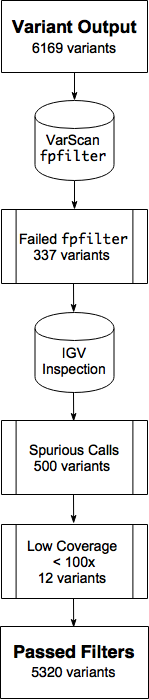
\includegraphics[scale=0.5]{variant_output.png}
	\caption{Add caption.}
	\label{fig:variant_output}
\end{figure}

%%%%%%%%%%%%%%%%%%%%%%%%%%%%%%%%%%%%%%%%%%%%%%%%%%%%%%%%%%%%%%%%%%%%%%
\subsection*{Germline variants are highly concordant between blood and FFPE specimens}

\begin{figure}[!h]
\centering
	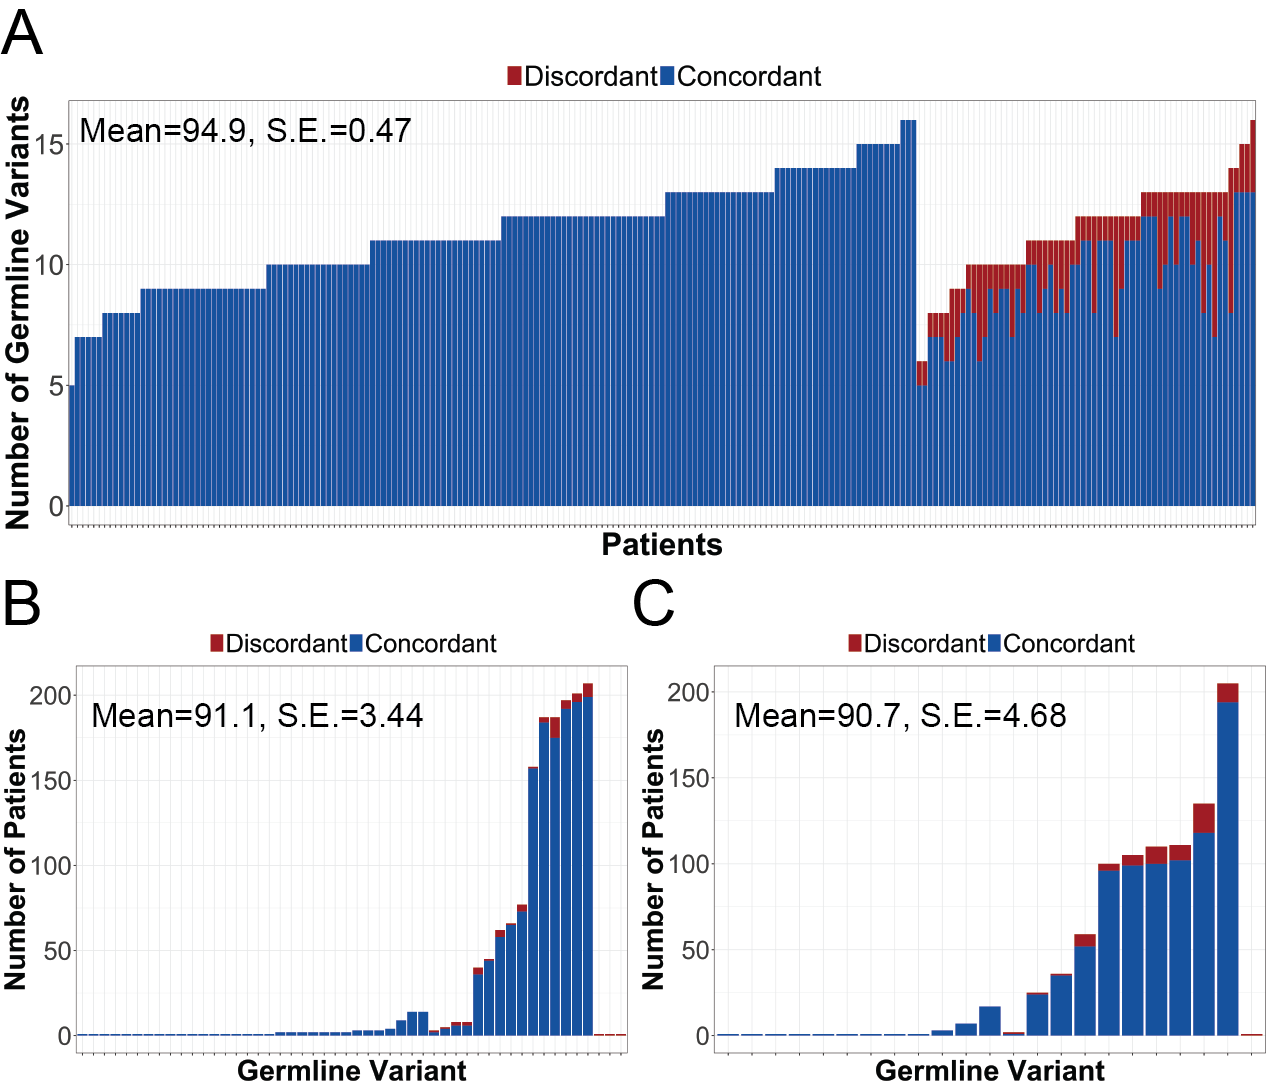
\includegraphics[scale=0.5]{true_positive_rate_variants.png}
	\caption{Add caption.}
	\label{fig:true_positive_rate_variants}
\end{figure}

%%%%%%%%%%%%%%%%%%%%%%%%%%%%%%%%%%%%%%%%%%%%%%%%%%%%%%%%%%%%%%%%%%%%%%
\subsection*{Reduced sensitivity is observed for detection of germline variants in FFPE specimens compared to blood}

\begin{figure}[!h]
	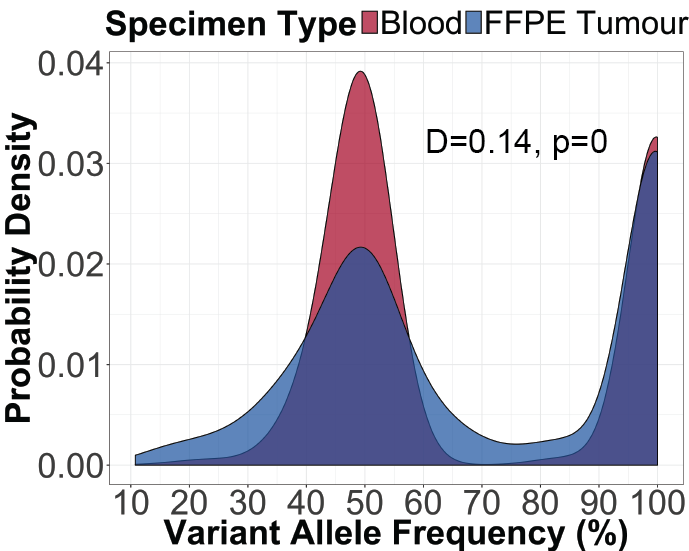
\includegraphics[scale=0.5]{germline_vaf_sens.png}
	\caption{Add caption.}
	\label{fig:germline_vaf_sens}
\end{figure}

\begin{table}[H]
\caption{Sensitivity of detecting germline variants in blood and FFPE specimens at various variant allele frequency thresholds.}
\label{sensitivity}
\centering
      \begin{tabular}{cllcclllccl}
        \hline
				\multicolumn{1}{l}{ }
				&
				\multicolumn{4}{l}{Blood}
				&&
				\multicolumn{4}{l}{FFPE Tumour}
        \\
				\cline{2-5}\cline{7-10}
        VAF (\%) & FN\mbox{*} & TP\mbox{**} & Sensitivity & 95\% CI && FN\mbox{*} & TP\mbox{**} & Sensitivity & 95\% CI
        \\
        \hline
        10 & 0 & 2461 & 1.0 & 1.0--1.0 && 0 & 2428 & 1.0 & 1.0--1.0
        \\
        15 & 2 & 2459 & 1.0 & 1.0-1.0 && 12 & 2416 & 1.0 & 0.99--1.0
        \\
        20 & 3 & 2458 & 1.0 & 1.0--1.0 && 48 & 2380 & 0.98 & 0.97--0.99
        \\
        25 & 15 & 2446 & 0.99 & 0.99--1.00 && 79 & 2349 & 0.97 & 0.96--0.97
        \\
        30 & 20 & 2441 & 0.99 & 0.99--1.00 && 121 & 2307 & 0.95 & 0.94--0.96
        \\
        35 & 33 & 2428 & 0.99 & 0.98--0.99 && 197 & 2231 & 0.92 & 0.91--0.93
        \\
        40 & 107 & 2354 & 0.96 & 0.95--0.96 && 328 & 2100 & 0.86 & 0.85--0.88
        \\
        45 & 234 & 2227 & 0.90 & 0.89--0.92 && 470 & 1958 & 0.81 & 0.79--0.82
        \\
				\hline
      \end{tabular} \\
\end{table}

%%%%%%%%%%%%%%%%%%%%%%%%%%%%%%%%%%%%%%%%%%%%%%%%%%%%%%%%%%%%%%%%%%%%%%
\subsection*{High positive predictive value can be achieved for referral of potential germline variants to downstream confirmatory testing}

\begin{figure}[!h]
	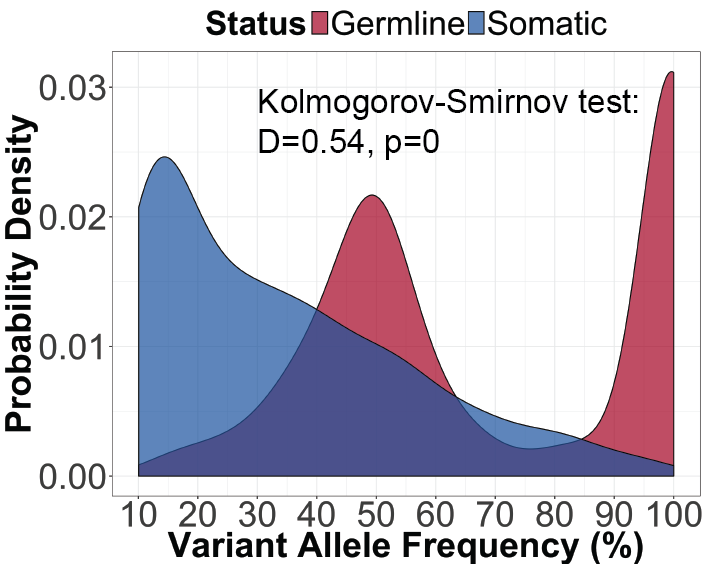
\includegraphics[scale=0.5]{germline_somatic_ppv.png}
	\caption{Add caption.}
	\label{fig:germline_somatic_ppv}
\end{figure}

\begin{table}[H]
\caption{Positive predictive value for referral of potential germline variants for downstream confirmatory testing.}
\label{ppv}
\centering
      \begin{tabular}{ccccccl}
        \hline
        VAF (\%) & False Positive & True Positive & Total Calls & Positive Predictive Value & 95\% CI
        \\
        \hline
        10 & 431 & 2428 & 2859 & 0.85 & 0.84--0.86
        \\
        15 & 319 & 2416 & 2735 & 0.88 & 0.87--0.90
        \\
        20 & 273 & 2380 & 2653 & 0.90 & 0.88--0.91
        \\
        25 & 245 & 2349 & 2594 & 0.91 & 0.89--0.92
        \\
        30 & 203 & 2307 & 2510 & 0.92 & 0.91--0.93
        \\
        35 & 178 & 2231 & 2409 & 0.93 & 0.91--0.94
        \\
        40 & 146 & 2100 & 2246 & 0.93 & 0.92--0.94
        \\
        45 & 118 & 1958 & 2076 & 0.94 & 0.93--0.95
        \\
				\hline
      \end{tabular} \\
\end{table}

\section*{Discussion}

\section*{Conclusions}

%%%%%%%%%%%%%%%%%%%%%%%%%%%%%%%%%%%%%%%%%%%%%%
%%                                          %%
%% Backmatter begins here                   %%
%%                                          %%
%%%%%%%%%%%%%%%%%%%%%%%%%%%%%%%%%%%%%%%%%%%%%%

\begin{backmatter}

\section*{Competing interests}
  The authors declare that they have no competing interests.

\section*{Author's contributions}
    Text for this section \ldots

\section*{Acknowledgements}
  Text for this section \ldots
%%%%%%%%%%%%%%%%%%%%%%%%%%%%%%%%%%%%%%%%%%%%%%%%%%%%%%%%%%%%%
%%                  The Bibliography                       %%
%%                                                         %%
%%  Bmc_mathpys.bst  will be used to                       %%
%%  create a .BBL file for submission.                     %%
%%  After submission of the .TEX file,                     %%
%%  you will be prompted to submit your .BBL file.         %%
%%                                                         %%
%%                                                         %%
%%  Note that the displayed Bibliography will not          %%
%%  necessarily be rendered by Latex exactly as specified  %%
%%  in the online Instructions for Authors.                %%
%%                                                         %%
%%%%%%%%%%%%%%%%%%%%%%%%%%%%%%%%%%%%%%%%%%%%%%%%%%%%%%%%%%%%%

% if your bibliography is in bibtex format, use those commands:
\bibliographystyle{bmc-mathphys} % Style BST file (bmc-mathphys, vancouver, spbasic).
\bibliography{/Users/evayap/Documents/biblitex_mendeley/pgx_ms.bib}      % Bibliography file (usually '*.bib' )
% for author-year bibliography (bmc-mathphys or spbasic)
% a) write to bib file (bmc-mathphys only)
% @settings{label, options="nameyear"}
% b) uncomment next line
%\nocite{label}

% or include bibliography directly:
% \begin{thebibliography}
% \bibitem{b1}
% \end{thebibliography}

%%%%%%%%%%%%%%%%%%%%%%%%%%%%%%%%%%%
%%                               %%
%% Figures                       %%
%%                               %%
%% NB: this is for captions and  %%
%% Titles. All graphics must be  %%
%% submitted separately and NOT  %%
%% included in the Tex document  %%
%%                               %%
%%%%%%%%%%%%%%%%%%%%%%%%%%%%%%%%%%%

%%
%% Do not use \listoffigures as most will included as separate files

\section*{Figures}
  \begin{figure}[h!]
  \caption{\csentence{Sample figure title.}}
      \end{figure}

\begin{figure}[h!]
  \caption{\csentence{Sample figure title.}
      Figure legend text.}
      \end{figure}

%%%%%%%%%%%%%%%%%%%%%%%%%%%%%%%%%%%
%%                               %%
%% Tables                        %%
%%                               %%
%%%%%%%%%%%%%%%%%%%%%%%%%%%%%%%%%%%

%% Use of \listoftables is discouraged.
%%
\section*{Supplementary Tables}

\normalsize
\begin{table}[H]
    \caption{Gene Reference Models for Genes in the OncoPanel.}\label{genemodel}
    \centering
    \begin{tabular}{ l l l }
		\hline
    Gene & Protein & Reference Model \\
		\hline
    AKT1 & Protein kinase B & NM\_001014431.1 \\
    ALK & Anaplastic lymphoma receptor tyrosine kinase & NM\_004304.3 \\
    BRAF & Serine/threonine-protein kinase B-Raf & NM\_004333.4 \\
    DPYD & Dihydropyrimidine dehydrogenase & NM\_000110.3 \\
    EGFR & Epidermal growth factor receptor & NM\_005228.3 \\
    ERBB2 & Receptor tyrosine-protein kinase erbB-2 & NM\_001005862.1 \\
    GSTP1 & Glutathione S-rransferase pi 1 & NM\_000852.3 \\
    HRAS & GTPase HRas & NM\_005343.2 \\
    IDH1 & Isocitrate dehydrogenase 1 & NM\_005896.2 \\
    IDH2 & Isocitrate dehydrogenase 2 & NM\_002168.2 \\
    KIT & Tyrosine-protein kinase Kit & NM\_000222.2 \\
    KRAS & KRas proto-oncogene GTPase & NM\_033360.2 \\
    MAPK1 & Mitogen-activated protein kinase 1 & NM\_002745.4 \\
    MAP2K1 & Mitogen-activated protein kinase kinase 1 & NM\_002755.3 \\
    MTHFR & Methylenetetrahydrofolate reductase & NM\_005957.4 \\
    MTOR & Serine/threonine-protein kinase mTOR & NM\_004958.3 \\
    NRAS & Neuroblastoma RAS viral oncogene homolog & NM\_002524.3 \\
    PDGFRA & Platelet-derived growth factor receptor alpha & NM\_006206.4 \\
    PIK3CA & Phosphatidylinositol-4,5-bisphosphate 3-kinase catalytic subunit alpha & NM\_006218.2 \\
    PTEN & Phosphatase and tensin homolog & NM\_000314.4 \\
    STAT1 & Signal transducer and activator of transcription 1 & NM\_007315.3 \\
    STAT3 & Signal transducer and activator of transcription 3 & NM\_139276.2 \\
    TP53 & Tumor protein P53 & NM\_000546.5 \\
    TYMP & Thymidine phosphorylase & NM\_001113755.2 \\
    TYMS & Thymidylate synthetase & NM\_001071.2 \\
    UGT1A1 & Uridine diphosphate (UDP)-glucuronosyl transferase 1A1 & NM\_000463.2\\
    \hline
    \end{tabular}
\end{table}

%%%%%%%%%%%%%%%%%%%%%%%%%%%%%%%%%%%
%%                               %%
%% Additional Files              %%
%%                               %%
%%%%%%%%%%%%%%%%%%%%%%%%%%%%%%%%%%%

\section*{Additional Files}
  \subsection*{Additional file 1 --- Sample additional file title}
    Additional file descriptions text (including details of how to
    view the file, if it is in a non-standard format or the file extension).  This might
    refer to a multi-page table or a figure.

  \subsection*{Additional file 2 --- Sample additional file title}
    Additional file descriptions text.


\end{backmatter}
\end{document}

\endinput
\subsection*{Frequency of germline and somatic variants detected in FFPE tumours}
This section will present the variant filtering procedure and categorization of the results, including germline, somatic, spurious, VarScan fpfilter, and PGx variants(?).

\begin{table}[htb]
\caption{Frequency of germline and somatic variants detected in the tumours of 213 patients in the TOP cohort.}\label{metrics}
\centering
\begin{tabular}{lcclcl}
        \hline
        Gene & Germline & Pathogenic Germline && Somatic \\
				 & (N Patients) & (N Patients) && (N Patients) \\
				\hline
				\\
				\multicolumn{1}{l}{\textit{Cancer predisposing}}
				&
				\multicolumn{2}{l}{ }
				&&
				\multicolumn{1}{l}{} \\
				\hline
				AKT1 & 0 & 0 && 2 (2) \\
				\arrayrulecolor{evagrey}\hline
				ALK & 1 (1) & 1 (1) && 2 (1) \\
				\hline
				BRAF & 0 & 0 && 18 (17) \\
				\hline
				EGFR & 170 (164) & 5 (5) && 31 (24) \\
				\hline
				HRAS & 0 & 0 && 1 (1) \\
				\hline
				MAP2K1 & 0 & 0 && 2 (2) \\
				\hline
				MAPK1 & 17 (17) & 3 (3) && 3 (2) \\
				\hline
				MTOR & 763 (213) & 6 (6) && 71 (30) \\
				\hline
				NRAS & 0 & 0 && 8 (8) \\
				\hline
				PDGFRA & 242 (185) & 0 && 8 (4) \\
				\hline
				PIK3CA & 0 & 0 && 15 (4) \\
				\hline
				PTEN & 0 & 0 && 1 (1) \\
				\hline
				STAT1 & 54 (51) & 1 (1) && 7 (6) \\
				\hline
				STAT3 & 10 (10) & 4 (4) && 16 (11) \\
				\hline
				TP53 & 189 (184) & 2 (2) && 131 (109) \\
				\arrayrulecolor{black}\hline
				\\
				\multicolumn{1}{l}{\textit{Pharmacogenomics}}
				&
				\multicolumn{2}{l}{ }
				&&
				\multicolumn{1}{l}{} \\
				\arrayrulecolor{black}\hline
				DPYD & 271 (212) & 1 (1) && 1 (1) \\
				\arrayrulecolor{evagrey}\hline
				GSTP1 & 106 (106) & 0 && 0 \\
				\hline
				MTHFR & 209 (177) & 0 && 0 \\
				\hline
				TYMP & 81 (76) & 2 (2) && 18 (13)\\
				\hline
				TYMS & 131 (131) & 0 && 0 \\
				\hline
				UGT1A1 & 96 (96) & 0 && 1 (1) \\
				\arrayrulecolor{black}\hline \\
				\\
				Total & 2396 (213*) & 25 (23*) && 431 (180) \\
				\arrayrulecolor{black}\hline
      \end{tabular}
\end{table}

\subsection*{High sensitivity and positive predictive value for germline variant calling in FFPE tumours can be achieved through applying variant allele frequency thresholds}
This section will show the calculation of sensitivity and PPV at different VAF thresholds.

\subsection*{Germline variants are highly concordant between blood and FFPE tumours}
PGx variants are highly concordant.

\subsection*{What are the causes of discordant variants?}
Low coverage sites, poor quality sites, LOH, formalin artifacts?

--

\subsection*{Study Design}
This study involved retrospective analysis of tumour-normal sequencing data from 213 patients diagnosed with various advanced cancers. The matched normal specimens for this study were derived from peripheral blood, which served as controls for assessment of formalin-induced DNA damages in FFPE tumours and gold standard specimens for detecting germline variants.

\paragraph*{Sub-sub-sub heading for section}
Text for this sub-sub-sub-heading \ldots

\section*{Orphaned Text}

\subsection*{Comparison of Amplicon Generation, Sequencing Results, and Coverage Statistics between Blood and FFPE Specimens}

Formalin fixation causes various types of DNA damage that can compromise DNA sequencing, including molecular testing with NGS approaches. Hence, we determined whether FFPE DNA is a reliable source for germline testing by comparing several NGS quality metrics between blood and FFPE tumours (\autoref{metrics}). As DNA fragmentation in FFPE specimens can result in reduced template DNA for amplicon generation, we compared the amount of amplicon generated between blood and FFPE tumours. We found a significant difference in the distributions of amplicon yield between specimen types (Wilcoxon signed-rank test, W=\num{23613}, \textit{P}\textless \num{2.2e-16}). Although the amount of DNA input for amplicon generation was also significantly different between blood and FFPE tumours (Wilcoxon signed-rank test, W=15004, \textit{P}=\num{3.5e-4}), Spearman's correlation showed that amplicon yield was weakly correlated with DNA input for amplicon generation (blood, \textit{r}=0.29, 95\% CI=0.16--0.40, \textit{P}=\num{2.1e-5}; FFPE tumour, \textit{r}=0.25, 95\% CI=0.12--0.37, \textit{P}=\num{2.5e-4}). This result implies that the difference in amplicon yield is contributed by specimen type with FFPE tumours demonstrating a lower median amplicon yield of 103.6 ng (range: 11.6--325.5 ng) than the median amplicon yield of blood, which is 299.2 ng (range: 84.0--1438.0 ng).

Furthermore, we compared read alignment between blood and FFPE libraries to examine whether the different specimen types result in comparable sequencing data. For the proportion of on-target aligned reads, which are reads that aligned to target regions used for variant calling, we found no significant difference in distributions between blood and FFPE tumours (Wilcoxon signed-rank test, W=\num{10178.5}, \textit{P}=\num{9.4e-2}). Similarly, no significant difference in the proportion of off-target aligned reads (i.e. reads that mapped to the human reference genome but not to target regions) was demonstrated between blood and FFPE tumours (Wilcoxon signed-rank test, W=\num{11494.5}, \textit{P}=\num{0.7}). However, differences in the proportions of unaligned and contaminant reads were significant between specimen types (Wilcoxon signed-rank test, unaligned: W=\num{19069}, \textit{P}=\num{5.2e-15}; contaminant: W=\num{14877}, \textit{P}=\num{9.9e-4}). While NGS libraries generated from blood and FFPE DNA differed in proportions of unaligned and contaminant reads, their libraries resulted in comparable proportions of on-target aligned reads, thereby providing equivalent amount of usable sequencing data for variant calling.

To assess the uniformity of coverage depth in blood and FFPE tumours, we measured the percentage of high quality target bases (Phred-scaled base quality score $\geq$20) with zero, $\geq$100x, and $\geq$1000x coverage depth for all libraries. Out of 431 libraries, only two libraries, one blood and one FFPE tumour, contained target bases with zero coverage depth, in which 0.006\% and 0.4\% of target bases have zero coverage depth for the blood library and FFPE library respectively. While we observed no significant difference in the percentage of target bases with $\geq$100x coverage depth (Wilcoxon signed-rank test, W=\num{243}, \textit{P}=\num{0.58}), we revealed a significant difference in the percentage of target bases with $\geq$1000x coverage depth between specimen types (Wilcoxon signed-rank test, W=\num{7268}, \textit{P}=\num{1.92e-5}). This finding shows that FFPE libraries are comprised of lower proportions of target bases with high coverage depth (i.e. 1000x) than blood libraries, in which the median percentage of $\geq$1000x target bases for FFPE libraries is 99.98\% (range: 20.61--100.00\%), whereas the median percentage of $\geq$1000x target bases for blood libraries is 100.00\% (range: 99.00--100.00\%).

Work on the summary later \ldots

Together, our comparisons of several NGS quality metrics reveal that formalin fixation can interfere with amplicon generation and sequencing depth, whereas its effect on on-target aligned reads remains negligible.

\subsection*{Evaluation of Amplicon Performance between Specimen Types}

Increased DNA fragmentation in FFPE specimens can result in lower coverage depth for longer amplicons, causing amplicon performance to vary between blood and FFPE tumours. To assess this discrepancy, we normalized coverage depth for all 416 amplicons in the OncoPanel to remove library size bias and compared the normalized coverage depth for each amplicon between blood and FFPE specimens. Using the Wilcoxon signed-rank test with Benjamini-Hochberg multiple hypothesis correction, we identified 369 out of 416 amplicons, which is 88.7\% of OncoPanel amplicons, that demonstrated significant differences in normalized coverage depth between specimen types (\textit{P}\textless \num{0.05}). Out of these 369 amplicons, 241 amplicons (65.3\% of amplicons that significantly differed in normalized coverage depth) presented higher median normalized coverage depths in blood than in FFPE tumours.

We next examined whether the differences in amplicon performance stem from amplicon length. For each amplicon, we calculated the percentage of libraries that met the coverage depth thresholds of $\geq$100x, $\geq$200x, $\geq$300x, $\geq$400x, and $\geq$500x, which we considered as parameters that reflected amplicon performance. Using the Spearman's correlation, we showed that amplicon performance negatively correlates with amplicon length in FFPE specimens (\textit{P}\textless \num{0.05}), whereas very weak correlations were revealed in blood specimens (Insert figure). Our observation indicates that DNA fragmentation as a result of formalin fixation, which causes discrepancy in the integrity of template DNA between blood and FFPE samples, is a probable cause of reduced amplicon performance for increased amplicon length in FFPE specimens.

Aside from amplicon length, amplicons in the OncoPanel also vary in GC content. As GC-rich and AT-rich regions are known to pose sequencing difficulties, we evaluated the effect of sequence complexity on amplicon performance using the Spearman's correlation (Insert figure).

Insert RepeatMasker results, Spearman's analysis does not make sense here but can be included in thesis etc., and work on the summary later \ldots

\subsection*{Assessment of Sequence Artifacts Induced by Formalin Fixation}
In addition to fragmentation damages in DNA, formalin fixation also induces sequence artifacts, particularly C$>$T/G$>$A transitions as a result of deamination of cytosine bases. To evaluate the prevalence of sequence artifacts in FFPE specimens, we measured the fraction of nucleotide changes for non-variant sites within the variant allele frequency ranges of 1--10\% and 11-25\%.

\textbf{In this section, I want to show that FFPE specimens have more artifactual sequence alterations compared to blood, particularly at low allele frequency. Using the replicates, I will further show that the sequence artifacts occur at low allele frequency as well. Next, TsTv ratios can be used as an indicator for "bad" FFPE samples.}

\subsection*{Correlation of Age of Paraffin Blocks and The Extent of Formalin-induced DNA Damages}

Herein, I'll show that older the paraffin block, the more extensive the DNA damages.
